\documentclass[11pt,aspectratio=169]{beamer}

\usepackage[T1]{fontenc}
\usepackage[utf8]{inputenc}
\usepackage[british]{babel}
\usepackage{lmodern}
\usepackage{graphicx}
\usepackage{booktabs}
\graphicspath{{talk/assets/}{assets/}}
\usepackage{pgfplots}
\pgfplotsset{compat=1.18}

% White background and dark text; colour distinguishes chart data and table values.
\definecolor{charcoal}{HTML}{252A2D}
\definecolor{teal}{HTML}{21736F}
\definecolor{muted}{HTML}{626A70}
\definecolor{chartorange}{HTML}{B16B24}
\definecolor{chartblue}{HTML}{4267A0}
\definecolor{chartpurple}{HTML}{8B5A8B}
\definecolor{assumptionred}{HTML}{B04E43}
\setbeamercolor{normal text}{fg=charcoal,bg=white}
\setbeamercolor{structure}{fg=charcoal}
\setbeamercolor{frametitle}{fg=charcoal,bg=white}
\setbeamercolor{title}{fg=charcoal}
\setbeamercolor{page number in head/foot}{fg=muted}
\setbeamerfont{normal text}{size=\normalsize}
\setbeamerfont{frametitle}{size=\LARGE,series=\bfseries}
\setbeamerfont{title}{size=\fontsize{26}{31}\selectfont,series=\bfseries}
\setbeamerfont{page number in head/foot}{size=\scriptsize}
\setbeamersize{text margin left=11mm,text margin right=11mm}
\setbeamertemplate{navigation symbols}{}
\setbeamertemplate{headline}{}
\setbeamertemplate{itemize item}{\raisebox{0.15ex}{\scriptsize\textbullet}}
\setbeamertemplate{frametitle}{%
  \vspace{5mm}%
  \usebeamerfont{frametitle}\insertframetitle\par
  \vspace{2mm}%
}
\setbeamertemplate{footline}{%
  \hfill\usebeamerfont{page number in head/foot}%
  \usebeamercolor[fg]{page number in head/foot}%
  \insertframenumber\hspace{11mm}\vspace{4mm}%
}

\title{Agentic AI in\\mathematical research}
% Add author, affiliation and event details when they are settled.
\author{}
\date{}

% Editable data charts. Provenance and the source snapshot are in talk/sources/.
\pgfplotsset{intro chart/.style={
  width=\linewidth,height=40mm,
  scaled ticks=false,
  tick label style={font=\fontsize{7}{8.5}\selectfont},
  axis lines=left,axis line style={muted!45},
  tick style={muted!45},tick align=outside,
  ymajorgrids=true,grid style={muted!15},
  clip=false,
  legend style={draw=none,fill=none,font=\fontsize{7}{8.5}\selectfont,
    at={(0,-0.23)},anchor=north west,cells={anchor=west},
    row sep=1pt,inner sep=0pt},
}}

\begin{document}

\begin{frame}[plain]
  \vspace{10mm}
  {\usebeamerfont{title}\usebeamercolor[fg]{title}\inserttitle\par}
\end{frame}

\begin{frame}[t]{A brief disclaimer}
  I am not an expert in this field. I have been exploring it out of curiosity
  and to stay up to date.

  \vspace{3mm}
  This talk neither argues for nor argues against using AI to write papers.

  \vspace{3mm}
  \begin{itemize}
    \setlength{\itemsep}{3.5mm}
    \item A brief history and overview of mathematical research with LLMs,
      focusing on agentic approaches.
    \item What the literature tells us about successful approaches
      and their limitations.
    \item A case study where I build an AI research team to write a paper.
  \end{itemize}
\end{frame}

\begin{frame}[t]{AI use and mathematical output}
  \begin{columns}[T,onlytextwidth]
    \begin{column}{0.48\textwidth}
      {\small\bfseries AI disclosures on arXiv\par}
      {\fontsize{7.5}{9}\selectfont\color{muted}%
        Share of math-related submissions, 2026\par}
      \vspace{2mm}
      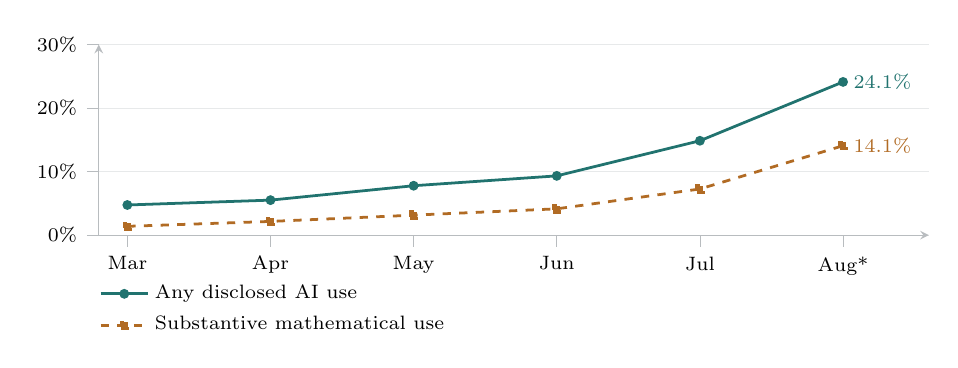
\begin{tikzpicture}
        \begin{axis}[intro chart,
          xmin=2.8,xmax=8.6,ymin=0,ymax=30,
          xtick={3,4,5,6,7,8},xticklabels={Mar,Apr,May,Jun,Jul,Aug*},
          ytick={0,10,20,30},yticklabel={\pgfmathprintnumber{\tick}\%},
          legend columns=1,
        ]
          % Numerators and denominators are from Jin, Ke and Sui, Table 1.
          \addplot[teal,line width=1pt,mark=*,mark size=1.25pt] coordinates
            {(3,4.74833808)(4,5.51304689)(5,7.78280543)(6,9.33508025)(7,14.86695545)(8,24.13639403)}
            node[pos=1,anchor=west,font=\fontsize{7.5}{9}\selectfont,text=teal] {24.1\%};
          \addlegendentry{Any disclosed AI use}
          \addplot[chartorange,dashed,line width=1pt,mark=square*,mark size=1.2pt] coordinates
            {(3,1.38651472)(4,2.15813223)(5,3.14932127)(6,4.14346544)(7,7.27103960)(8,14.08513483)}
            node[pos=1,anchor=west,font=\fontsize{7.5}{9}\selectfont,text=chartorange] {14.1\%};
          \addlegendentry{Substantive mathematical use}
        \end{axis}
      \end{tikzpicture}
    \end{column}
    \begin{column}{0.48\textwidth}
      {\small\bfseries Submissions by field\par}
      {\fontsize{7.5}{9}\selectfont\color{muted}%
        New preprints, January--August each year\par}
      \vspace{2mm}
      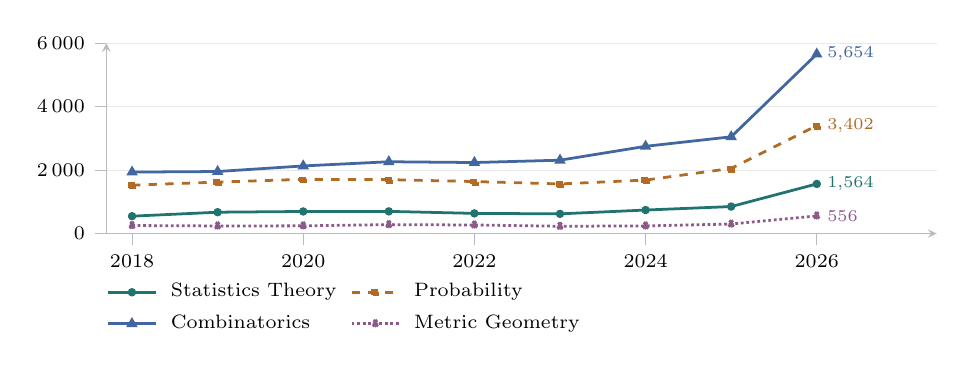
\begin{tikzpicture}
        \begin{axis}[intro chart,
          xmin=2017.7,xmax=2027.4,ymin=0,ymax=6000,
          xtick={2018,2020,2022,2024,2026},ytick={0,2000,4000,6000},
          xticklabel style={/pgf/number format/1000 sep={}},
          yticklabel style={/pgf/number format/1000 sep={\,}},
          legend columns=2,column sep=3pt,
        ]
          \addplot[teal,line width=1pt,mark=*,mark size=1pt] coordinates
            {(2018,548)(2019,673)(2020,696)(2021,699)(2022,636)(2023,621)(2024,741)(2025,851)(2026,1564)}
            node[pos=1,anchor=west,font=\fontsize{6.5}{8}\selectfont,text=teal] {1,564};
          \addlegendentry{Statistics Theory}
          \addplot[chartorange,dashed,line width=1pt,mark=square*,mark size=1pt] coordinates
            {(2018,1524)(2019,1622)(2020,1709)(2021,1699)(2022,1639)(2023,1564)(2024,1686)(2025,2052)(2026,3402)}
            node[pos=1,anchor=west,font=\fontsize{6.5}{8}\selectfont,text=chartorange] {3,402};
          \addlegendentry{Probability}
          \addplot[chartblue,line width=1pt,mark=triangle*,mark size=1.4pt] coordinates
            {(2018,1937)(2019,1955)(2020,2131)(2021,2263)(2022,2238)(2023,2312)(2024,2749)(2025,3049)(2026,5654)}
            node[pos=1,anchor=west,font=\fontsize{6.5}{8}\selectfont,text=chartblue] {5,654};
          \addlegendentry{Combinatorics}
          \addplot[chartpurple,densely dotted,line width=1pt,mark=diamond*,mark size=1.4pt] coordinates
            {(2018,253)(2019,240)(2020,243)(2021,282)(2022,270)(2023,230)(2024,241)(2025,301)(2026,556)}
            node[pos=1,anchor=west,font=\fontsize{6.5}{8}\selectfont,text=chartpurple] {556};
          \addlegendentry{Metric Geometry}
        \end{axis}
      \end{tikzpicture}
    \end{column}
  \end{columns}

  \vspace{2mm}
  {\fontsize{7}{8.5}\selectfont\color{muted}%
    Left: 3,575 of 32,944 preprints disclosed AI use. *August covers 1--20.\par
    Right: category counts for published arXiv papers.\par
    \vspace{1mm}
    \href{https://arxiv.org/html/2608.24961v1}{Jin, Ke \& Sui (2026), Table 1}
    \quad
    \href{https://rosie-0525.github.io/arxiv-statistics/}{Explore arXiv Math Pulse}
    \quad\href{https://github.com/rosie-0525/arxiv-statistics}{GitHub source}.\par}
\end{frame}

\begin{frame}[t]{(How) have you used AI in your research?}
  \noindent{\large Which is the highest level you have used?\par}
  \vspace{2mm}
  \noindent\makebox[\textwidth][c]{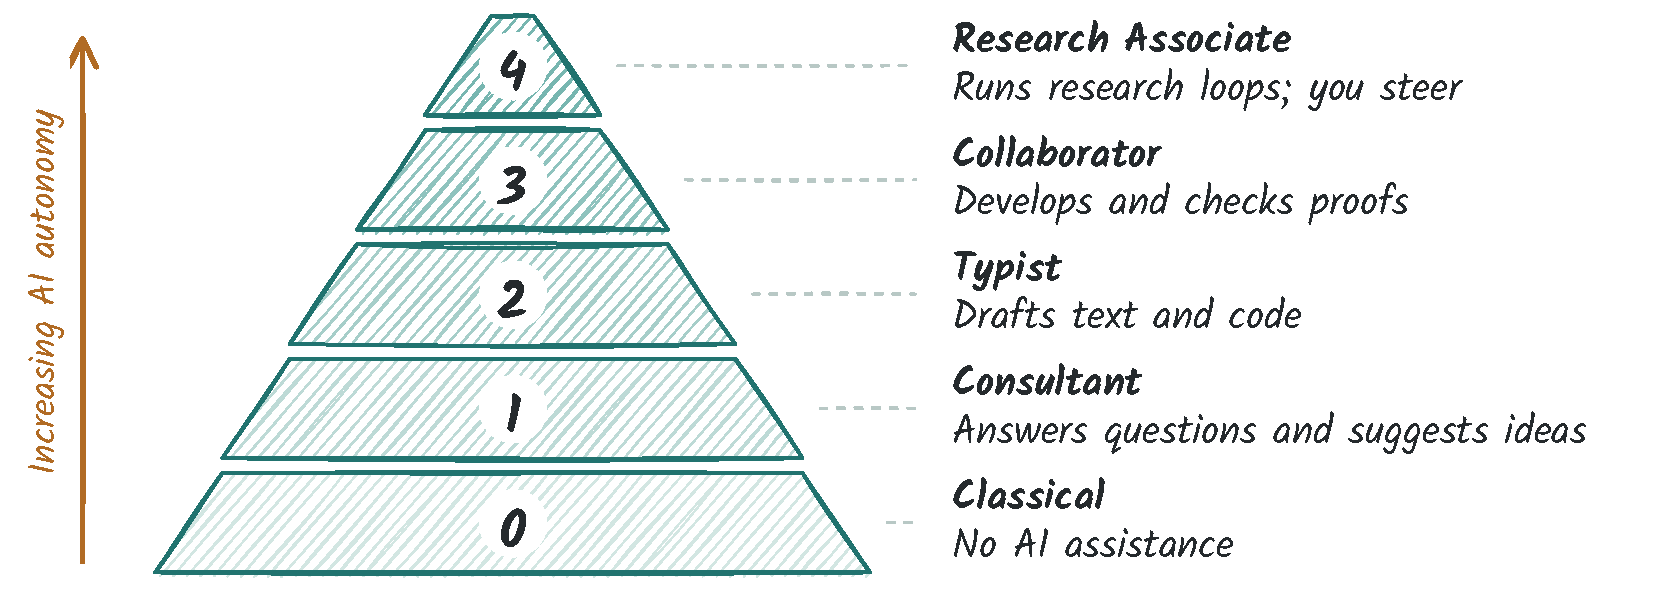
\includegraphics[clip,width=0.90\textwidth]{ai_usage_levels.pdf}}

  \vspace{2mm}
  {\fontsize{8}{10}\selectfont\color{muted}%
    Adapted from \href{https://arxiv.org/html/2603.15914v1\#S2}{%
      Zimmer et al. (2026), \emph{The Agentic Researcher}, Section 2}.\par}
\end{frame}

\section{A short history}
\begin{frame}[t]{A short history of math research with LLMs}
  \vspace{12mm}
  \noindent{\LARGE Agentic research systems over time \par}
  \vspace{5mm}
  {\large A brief history, with a focus on mathematics.\par}
\end{frame}

% Paper recaps place the short author-year citation in the title and a
% short description of the approach or the paper title directly underneath.
\begin{frame}[t]{FunSearch\quad{\fontsize{14}{17}\selectfont\mdseries%
  \href{https://doi.org/10.1038/s41586-023-06924-6}{Romera-Paredes et al., \emph{Nature} (2024)}}}
  \fontsize{9}{10.5}\selectfont
  \noindent{\fontsize{9}{11}\selectfont%
    An evolutionary approach with fixed evaluation criteria implemented in computer programs.\par}
  \vspace{0.5mm}
  \noindent\makebox[\textwidth][c]{%
    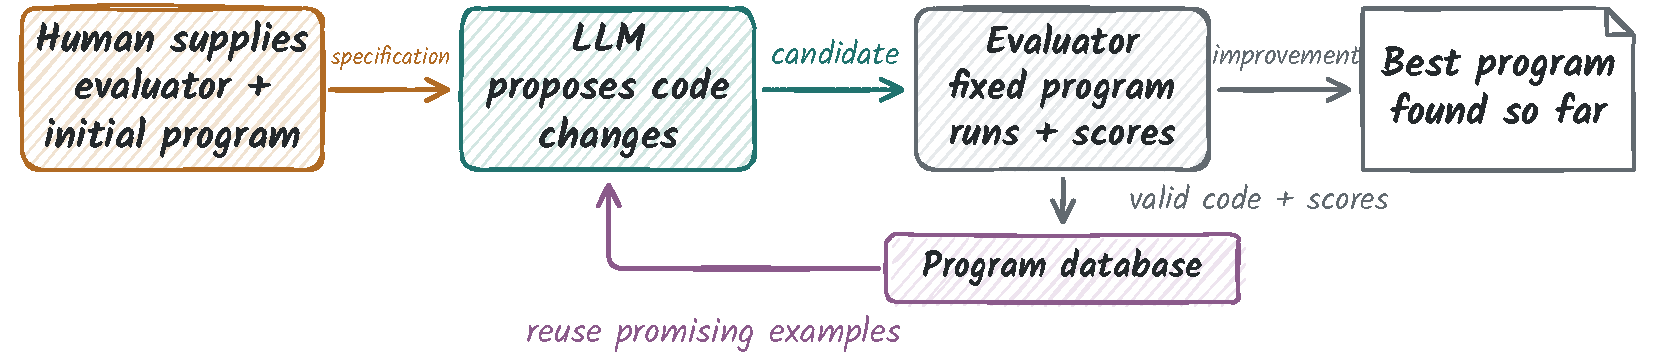
\includegraphics[clip,width=\textwidth,height=23mm,keepaspectratio]{funsearch_workflow.pdf}}\par
  \vspace{-2mm}
  \begin{columns}[T,onlytextwidth]
    \begin{column}{0.48\textwidth}
      {\fontsize{10}{12}\selectfont\bfseries Larger cap sets\par}
      \centering
      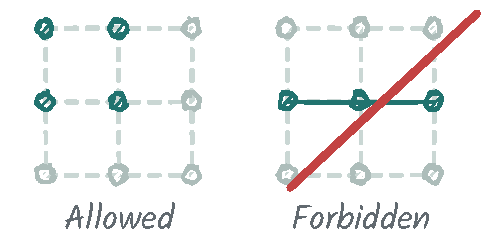
\includegraphics[clip,width=\linewidth,height=13mm,keepaspectratio]{funsearch_cap_set.pdf}\par
      \raggedright\fontsize{8.5}{10.5}\selectfont
      No three distinct points on a line in $\mathbb{F}_3^n$.\par
      In eight dimensions: 496 to 512 points.
    \end{column}
    \begin{column}{0.48\textwidth}
      {\fontsize{10}{12}\selectfont\bfseries Online bin-packing heuristics\par}
      \centering
      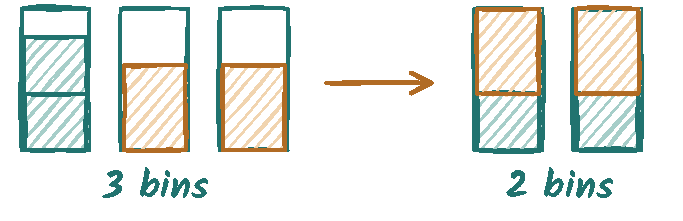
\includegraphics[clip,width=\linewidth,height=13mm,keepaspectratio]{funsearch_bin_packing.pdf}\par
      \raggedright\fontsize{8.5}{10.5}\selectfont
      The paper showed that the model can improve a standard heuristic such as best fit.
    \end{column}
  \end{columns}
  \vspace{1mm}
  {\fontsize{8}{9.5}\selectfont
    \href{https://arxiv.org/abs/2506.13131}{AlphaEvolve (2025)}
    later extended this approach: $4\times4$ complex matrix multiplication
    with 48 scalar multiplications, versus Strassen's 49.\par}
  \vspace{0.5mm}
  {\fontsize{6.8}{8}\selectfont%
    Workflow: Fig.~1; results: Fig.~4 and Table~1.
    \href{https://doi.org/10.1038/s41586-023-06924-6}{Romera-Paredes et al. (2024).}\par}
\end{frame}

\begin{frame}[t]{AlphaProof\quad{\fontsize{14}{17}\selectfont\mdseries%
  \href{https://doi.org/10.1038/s41586-025-09833-y}{Hubert et al., \emph{Nature} (2026)}}}
  \fontsize{9}{11}\selectfont
  \noindent{Another way to verify and evaluate mathematics is through formal verification in Lean.\par}
  \vspace{0mm}
  \noindent\makebox[\textwidth][c]{%
    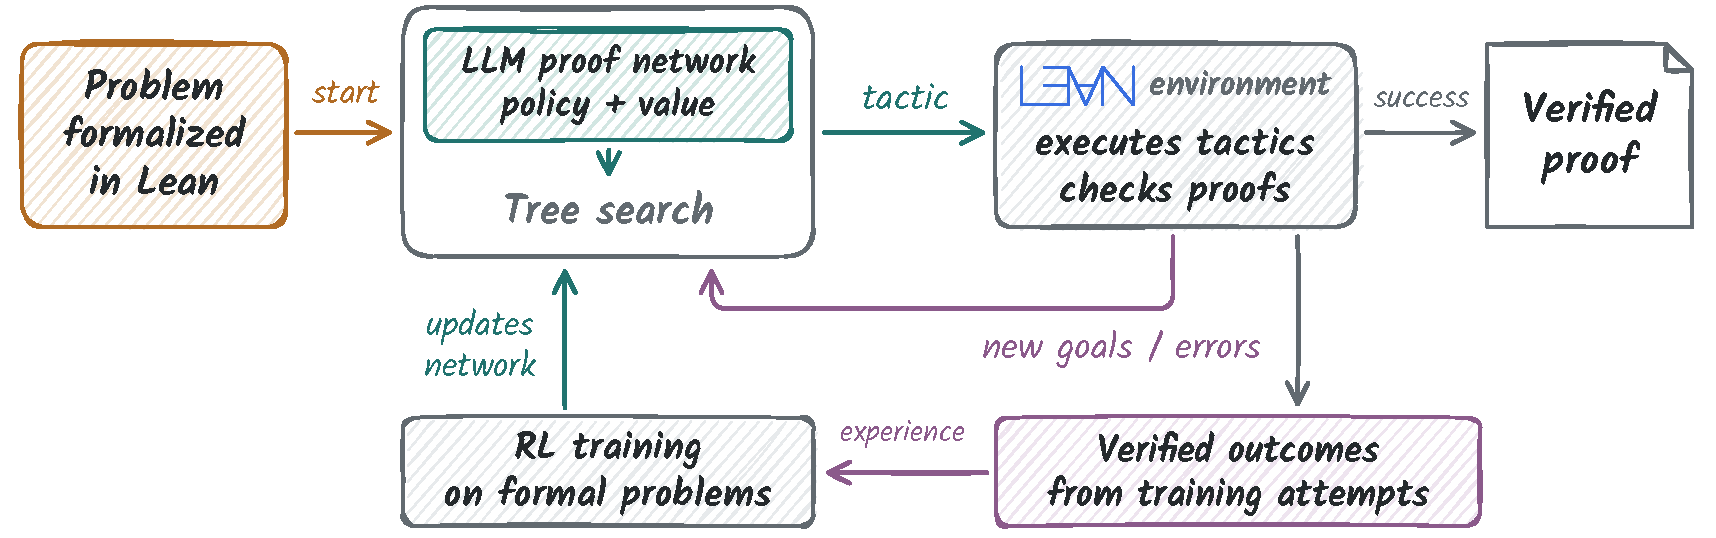
\includegraphics[clip,width=\textwidth,height=30mm,keepaspectratio]{alphaproof_architecture.pdf}}\par
  \vspace{1mm}
  \noindent\textbf{Function:} the model reads Lean goals and hypotheses. As output it proposes Lean tactics. Lean returns new proof states. This means it basically talks in Lean and gets Lean responses. \par
  \vspace{1mm}
  \noindent\textbf{Additional Learning:} the model learns from proof attempts through reinforcement learning.\par
  \vspace{1.5mm}
  \noindent{IMO 2024: 28/42 points, silver-medal level (AlphaProof: 3 problems; AlphaGeometry 2: 1).}\par
  \vspace{0mm}
  {\fontsize{7}{8.5}\selectfont%
    Figs.~1--2; AlphaProof and Training sections.
    \href{https://doi.org/10.1038/s41586-025-09833-y}{\emph{Nature} 651, 607--613 (2026).}\par}
  \note{The proof network generates Lean tactic code directly from the current
    proof state. Its policy proposes tactics and its value head estimates the
    remaining proof length; both guide tree search.
    Pretraining used about 300 billion tokens of code and mathematical text,
    followed by supervised fine-tuning on about 300,000 state--tactic pairs
    from human-written Mathlib proofs, then reinforcement learning.
    A separate fine-tuned Gemini 1.5 Pro model translated natural-language
    statements into Lean to create the training curriculum.
    Source: Hubert et al., \url{https://doi.org/10.1038/s41586-025-09833-y},
    Prover agent, Training, and Auto-formalization sections.}
\end{frame}

\begin{frame}[t]{Aletheia\quad{\fontsize{14}{17}\selectfont\mdseries%
  \href{https://arxiv.org/abs/2602.10177}{Feng et al., arXiv (2026)}}}
  \noindent{\fontsize{9}{11}\selectfont%
    We can also use an independent LLM for verification. This does not guarantee correctness.\par}
  \vspace{0mm}
  \begin{columns}[T,onlytextwidth]
    \begin{column}{0.49\textwidth}
      {\fontsize{10}{12}\selectfont\bfseries Gemini Deep Think agents}\par
      \vspace{1mm}
      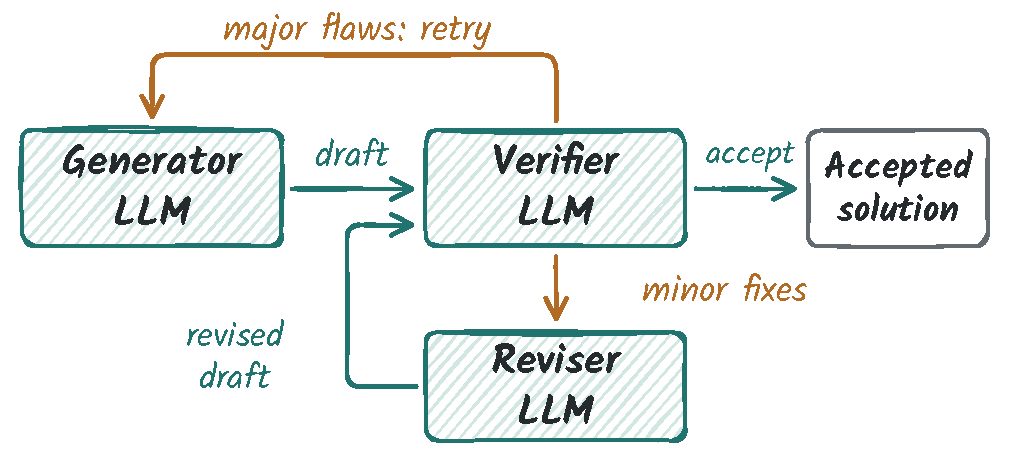
\includegraphics[clip,width=\linewidth,height=29mm,keepaspectratio]{aletheia_architecture.pdf}\par
      {\fontsize{7.5}{9}\selectfont%
        LLM judgment; no formal guarantee (Fig.~1).\par}
      \vspace{2mm}
      {\fontsize{9}{11}\selectfont
        {\bfseries Reported mathematical results}\par
        \vspace{1mm}
        \textbullet\ Erd\H{o}s: 2 full + 2 partial new solutions from 700 problems, checked by experts.\par}
    \end{column}
    \begin{column}{0.47\textwidth}
      \fontsize{8.3}{9.5}\selectfont
      {\fontsize{10}{12}\selectfont\bfseries Other LLM research systems}\par
      \vspace{1.5mm}
      \textbf{The AI Scientist}\quad
      \href{https://doi.org/10.1038/s41586-026-10265-5}{\emph{Nature} (2026)}\par
      Ran ML experiments and wrote a paper that passed a workshop's first review round.\par
      \vspace{1.5mm}
      \textbf{Google Co-Scientist}\quad
      \href{https://doi.org/10.1038/s41586-026-10644-y}{\emph{Nature} (2026)}\par
      Agents proposed and refined leukaemia drug combinations, validated in laboratory experiments.\par
      \vspace{1.5mm}
      \textbf{Virtual Lab}\quad
      \href{https://doi.org/10.1038/s41586-025-09442-9}{\emph{Nature} (2025)}\par
      LLM agents designed SARS-CoV-2 nanobodies with binding confirmed in laboratory tests.\par
      \vspace{1.5mm}
      \textbf{OpenAI: Navier--Stokes}\quad
      \href{https://openai.com/index/navier-stokes-solution/}{report (2026)}\par
      Different approaches explored with
      10,000 agents and human steering.\par
    \end{column}
  \end{columns}
\end{frame}

\section{Agentic systems}
\begin{frame}[t]{Agentic systems}
  \vspace{12mm}
  \noindent{\LARGE From LLMs to research teams\par}
\end{frame}

\begin{frame}[t]{Environment, context, tools and agents}
  \begin{columns}[T,onlytextwidth]
    \begin{column}{0.18\textwidth}
      \centering
      \vspace{3mm}
      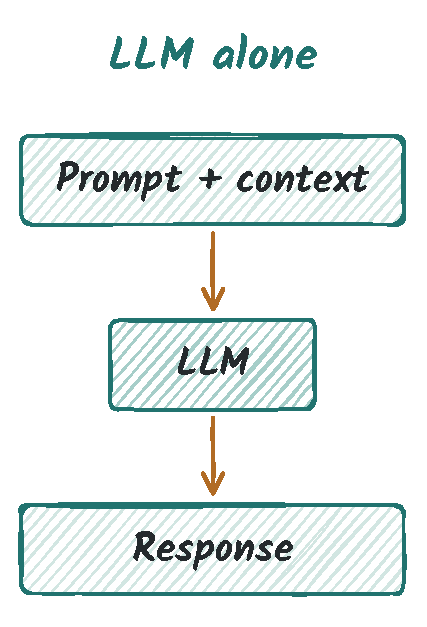
\includegraphics[clip,width=\linewidth,height=48mm,keepaspectratio]{llm_alone.pdf}\par
      \vspace{2mm}
      {\fontsize{9}{11}\selectfont $Y=f_\theta(p,c;\xi)$\par}
      \vspace{0.5mm}
      {\fontsize{7}{8.5}\selectfont
        $p$: prompt; $c$: context\par
        $\theta$: fixed model\par
        $\xi$: randomness\par}
    \end{column}
    \begin{column}{0.40\textwidth}
      \centering
      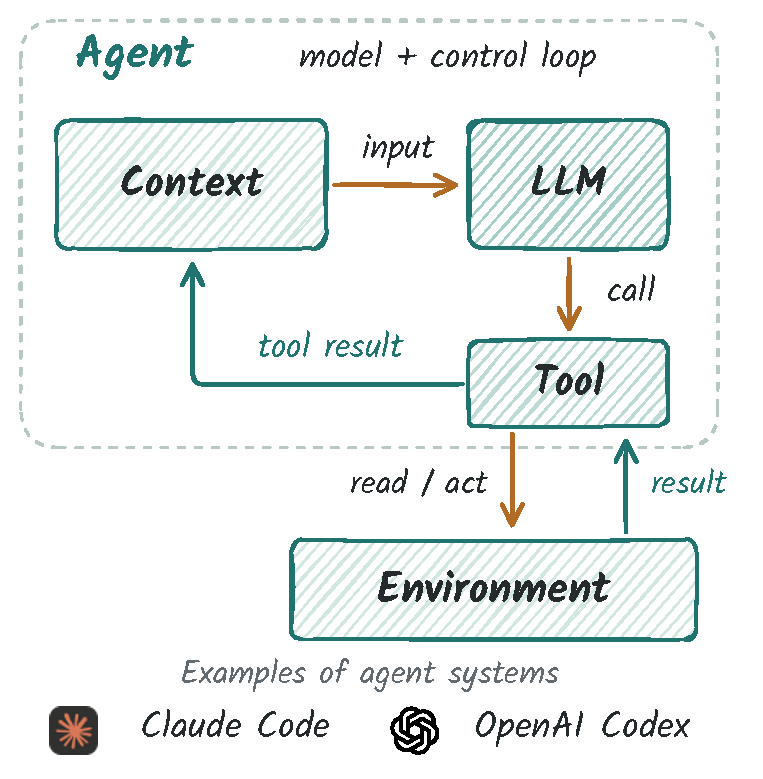
\includegraphics[clip,width=0.98\linewidth,height=54mm,keepaspectratio]{agent_components.pdf}
    \end{column}
    \begin{column}{0.38\textwidth}
      \fontsize{9}{10.5}\selectfont
      {\bfseries Environment}\par
      The workspace an agent can access:\par
      files, data, code and external services.\par
      \vspace{1.5mm}

      {\bfseries Context}\par
      The information given to the LLM.\par
      This includes instructions, messages and tool results.\par
      \vspace{1.5mm}

      {\bfseries Tool}\par
      An interface to observe or change the
      environment, e.g. PDF-reader or Python ...\par
      \vspace{1.5mm}

      {\bfseries Agent}\par
      An LLM-based system that uses tools
      and chooses its next step from results.\par
    \end{column}
  \end{columns}
  \vspace{1mm}
  {\fontsize{7}{8.5}\selectfont\color{muted}%
    Based on
    \href{https://developers.openai.com/api/docs/guides/agents-api/architecture}{OpenAI's Codex harness documentation}
    and \href{https://code.claude.com/docs/en/how-claude-code-works}{Claude Code's agentic loop}.\par}
\end{frame}

\begin{frame}[t]{Instructions and multi-agent systems}
  \begin{columns}[T,onlytextwidth]
    \begin{column}{0.37\textwidth}
      {\fontsize{11}{13}\selectfont\bfseries One agent\par}
      \vspace{1.5mm}
      \centering
      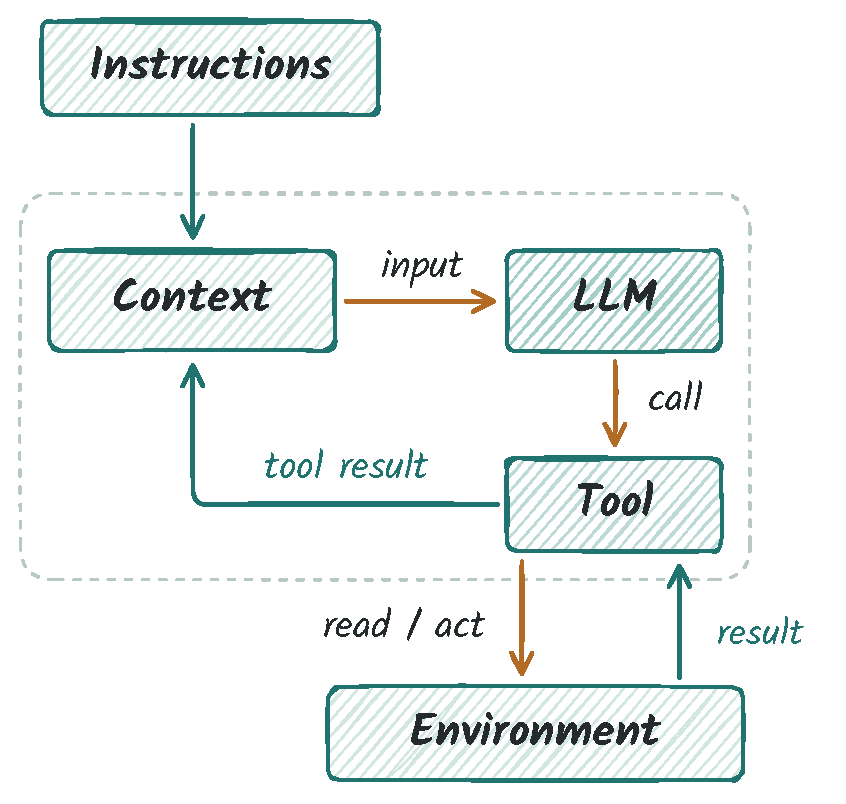
\includegraphics[clip,width=\linewidth,height=41mm,keepaspectratio]{skills_and_harness.pdf}
    \end{column}
    \begin{column}{0.60\textwidth}
      {\fontsize{11}{13}\selectfont\bfseries Several agents\par}
      \vspace{1.5mm}
      \centering
      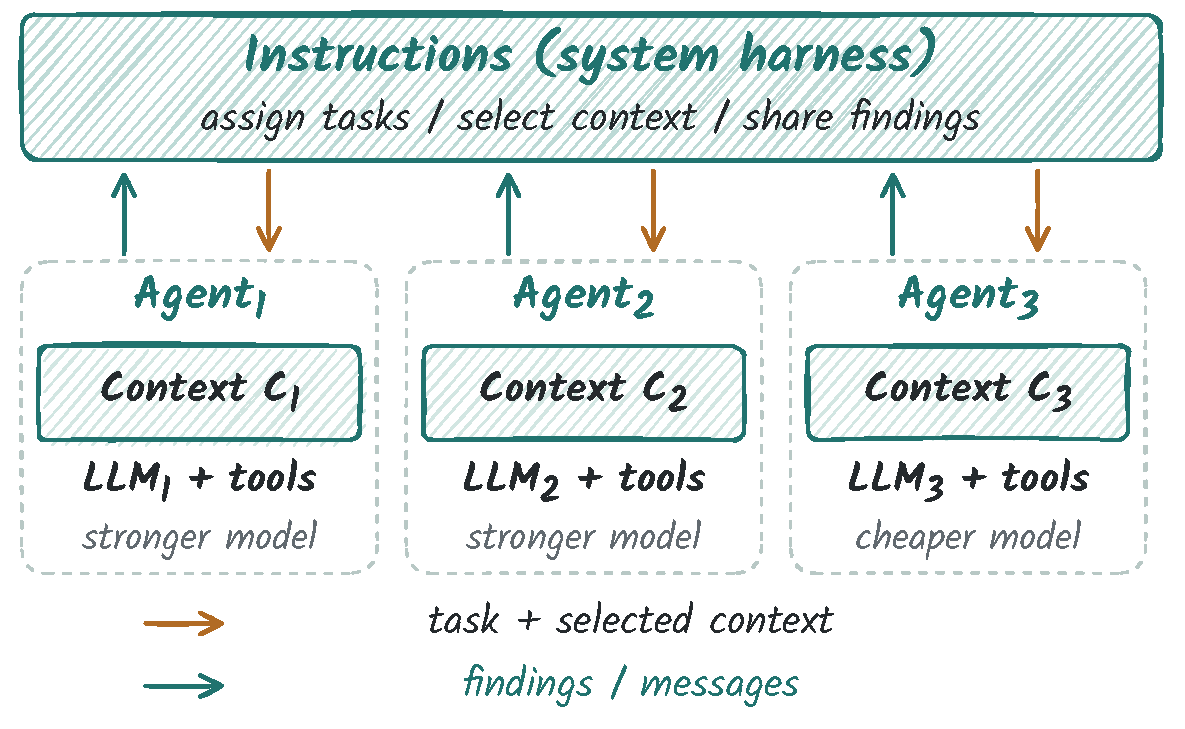
\includegraphics[clip,width=\linewidth,height=41mm,keepaspectratio]{multi_agent_contexts.pdf}
    \end{column}
  \end{columns}
  \vspace{1.5mm}
  {\fontsize{9}{10.5}\selectfont
    Each agent has its own context. Instructions specify its task and how it should work.\par
    \vspace{1mm}
    Communication is managed through \texttt{instructions.md} or the system harness.\par
    \vspace{1mm}
    More agents are not automatically better.\par}
  \note{Sources: ReAct (Yao et al., 2022), arXiv:2210.03629;
    AutoGen (Wu et al., 2023), arXiv:2308.08155.}
\end{frame}

\begin{frame}[t]{Why manage context and communication?}
  \noindent\begin{minipage}{\textwidth}
  \raggedright\fontsize{9}{10.4}\selectfont
  An LLM produces text $Y=f_{\theta}(p,c;\xi)$ whose distribution
  depends strongly on the context.\par
  \vspace{1.5mm}
  {\bfseries 1. Keep context focused}\quad
  {\fontsize{7}{8}\selectfont
    \href{https://aclanthology.org/2024.tacl-1.9/}{\color{muted}Liu et al. (2024)};
    \href{https://arxiv.org/html/2502.05167v3}{\color{muted}Modarressi et al. (2025)}}\par
  {\fontsize{8.5}{10}\selectfont%
  Give each agent the information it needs; long histories can obscure relevant details.\par
  This helps reduce distraction from irrelevant context.\par}
  \vspace{1mm}

  {\bfseries 2. Give review a fresh context}\quad
  {\fontsize{7}{8}\selectfont
    \href{https://arxiv.org/html/2310.13548v4}{\color{muted}Sharma et al. (2023)};
    \href{https://arxiv.org/html/2309.11495v2}{\color{muted}Dhuliawala et al. (2023)}}\par
  {\fontsize{8.5}{10}\selectfont%
  Review the draft and criteria without the writer's history; verify independently.\par
  This helps avoid repeating errors from the draft.\par}
  \vspace{1mm}

  {\bfseries 3. Match the model to the task}\quad
  {\fontsize{7}{8}\selectfont
    \href{https://arxiv.org/abs/2406.18665}{\color{muted}Ong et al., \emph{RouteLLM} (2024)}}\par
  Changing between stronger and cheaper models can improve the balance of cost and quality.\par
  \vspace{1mm}

  {\bfseries 4. Share findings and avoid duplicate work}\quad
  {\fontsize{7}{8}\selectfont
    \href{https://arxiv.org/abs/2305.14325}{\color{muted}Du et al. (2023)};
    \href{https://aclanthology.org/2025.acl-long.1170/}{\color{muted}Wang et al. (2025)}}\par
  Share useful results and redirect work that adds no new information.\par
  \vspace{1mm}

  {\bfseries 5. Explore distinct approaches independently}\quad
  {\fontsize{7}{8}\selectfont
    \href{https://aclanthology.org/2026.findings-acl.1694/}{\color{muted}Zhu et al. (2026)}}\par
  Especially important for mathematics since different starting points can lead to
  different proof strategies.\par
  \end{minipage}
\end{frame}

\section{A step-by-step research example}

\begin{frame}[t]{Agentic research: a worked example}
  \noindent{\large What do we need?\par}
  \vspace{3mm}
  \begin{itemize}
    \setlength{\itemsep}{2.5mm}
    \item An agent system: in my case, Codex.
    \item A precise mathematical problem statement.
    \item Relevant related work: definitions, known results and useful methods.
    \item \texttt{instruction.md}: the task, constraints and expected output.
    \item \texttt{skills.md}: an index of reusable methods and checks.
    \item \texttt{AGENTS.md}: standing project instructions for the agents.
  \end{itemize}

\end{frame}

\begin{frame}[t]{Step 1: Defining the problem}
  \begin{columns}[T,onlytextwidth]
    \begin{column}{0.65\textwidth}
      \raggedright\fontsize{9.5}{11}\selectfont
      A \textbf{simple point process} $X$ is a random set of distinct
      points in $\mathbb R^d$, finite in bounded regions.\par
      \vspace{1mm}
      Its count in a bounded Borel region $B$ is $X(B)=\#(X\cap B)$.\par
      \vspace{2mm}
      {\bfseries Stationarity} means that
      shifting all points leaves the distribution unchanged:\par
      \vspace{1mm}
      \noindent\makebox[\linewidth][c]{$\displaystyle X+t\overset{d}{=}X
        \quad\text{for every }t\in\mathbb R^d.$}\par
      \vspace{2mm}
      {\bfseries Homogeneous Poisson process, intensity $\lambda>0$}\par
      \begin{itemize}
        \setlength{\itemsep}{1mm}
        \item We demand that\par
          \noindent\makebox[\linewidth][c]{$X(B)\sim\operatorname{Poisson}(\lambda|B|),\quad
            \mathbb E[X(B)]=\lambda|B|.$}\par
        \item Counts in disjoint regions are independent.
        \item Therefore, for $B_1\cap B_2=\emptyset$,\par
          \noindent\makebox[\linewidth][c]{$\mathbb E[X(B_1)X(B_2)]
            =\mathbb E[X(B_1)]\mathbb E[X(B_2)].$}\par
      \end{itemize}
    \end{column}
    \begin{column}{0.31\textwidth}
      \centering
      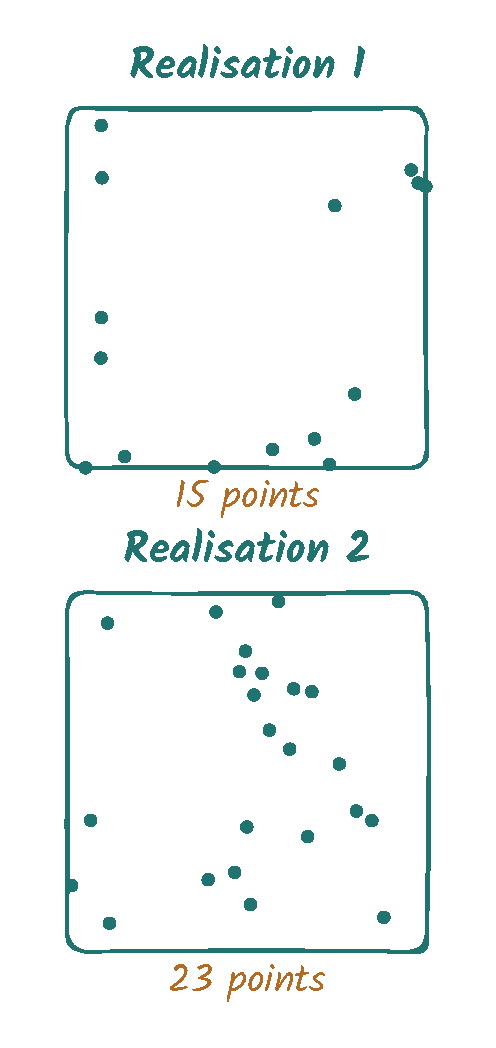
\includegraphics[clip,width=\linewidth,height=56mm,keepaspectratio]{poisson_teaching.pdf}\par
    \end{column}
  \end{columns}
  \vspace{1.5mm}
\end{frame}


\begin{frame}[t]{Step 1: Defining the Problem}
  \begin{columns}[T,onlytextwidth]
    \begin{column}{0.67\textwidth}
      \raggedright\fontsize{9.5}{11}\selectfont
      Under suitable assumptions, as disjoint sets $B_1,B_2$
      shrink to $x_1,x_2$,\par
      \vspace{1mm}
      \noindent\makebox[\linewidth][c]{$\displaystyle
        \frac{\mathbb{E}[X(B_1)X(B_2)]}
             {\mathbb{E}[X(B_1)]\,\mathbb{E}[X(B_2)]}
        \longrightarrow g_2(x_1,x_2).$}\par
           \vspace{1.5mm}
      More generally, for disjoint sets $B_1,\ldots,B_n$ shrinking to $x_1,\ldots,x_n$,\par
      \vspace{1mm}
      \noindent\makebox[\linewidth][c]{$\displaystyle
        \frac{\mathbb{E}[X(B_1)X(B_2)\cdots X(B_n)]}
             {\mathbb{E}[X(B_1)]\,\mathbb{E}[X(B_2)]\cdots \mathbb{E}[X(B_n)]}
        \longrightarrow g_n(x_1,x_2, \ldots , x_n).$}\par
      \vspace{1.5mm}
      This is the \textbf{$n$-point correlation function}: $g_n=\rho^{(n)}/\lambda^n$,\par
      where $\rho^{(n)}$ is the density of expected ordered distinct tuples.\par
      \vspace{1mm}
      Compared with Poisson at the same intensity:\par
      \vspace{1mm}
      {$g_n>1$: more such tuples.}\par
      {$g_n<1$: fewer such tuples.}\par
      $g_n=1$: the same local tuple density.\par
    \end{column}
    \begin{column}{0.30\textwidth}
      \centering
      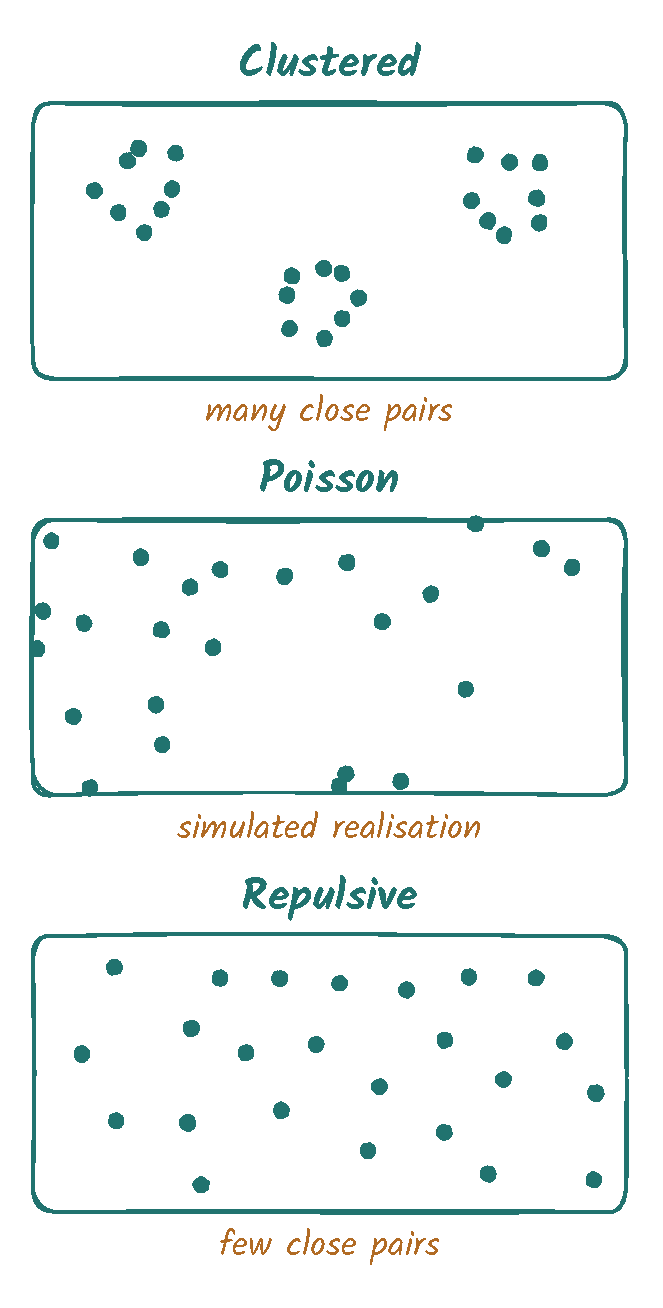
\includegraphics[clip,width=\linewidth,height=54mm,keepaspectratio]{point_process_patterns.pdf}\par
    \end{column}
  \end{columns}
  \vspace{0.5mm}

  \note{The cluster process has Poisson parents of intensity $\kappa=4$.
    Each parent has an independent Poisson number of offspring with mean $\mu=5$,
    independently and uniformly distributed in its disc of radius $a=0.10$.
    Only offspring are retained, so $\lambda=\kappa\mu=20$.
    If $A_a(r)$ is the overlap area of two radius-$a$ discs with centres distance $r$ apart,
    then $g_2(r)=1+A_a(r)/(\kappa(\pi a^2)^2)>1$ for $0<r<2a$;
    $g_2(r)=1$ for $r\geq2a$. See Baddeley, Example 2.12.
    For Mat\'ern II, start with Poisson proposals of intensity
    $\tau=-\log(1-20\pi h^2)/(\pi h^2)$, $h=0.11$, and independent uniform marks.
    Keep a proposal exactly when no proposal within distance $h$ has a smaller mark.
    The resulting intensity is $(1-e^{-\tau\pi h^2})/(\pi h^2)=20$.
    No two retained points are less than $h$ apart, hence $g_2(r)=0$ for $0<r<h$.
    No assertion that $g_2<1$ at all distances is intended.
    Both simulations use an outer buffer to give an exact restriction of the stationary process.}
\end{frame}
\begin{frame}[t]{Step 1: the precise problem}

  \noindent\begin{minipage}{\textwidth}
  \raggedright\fontsize{9.5}{11}\selectfont

 \textit{The conjecture is motivated by observed spatial correlations in earthquake catalogues. See
    \href{https://doi.org/10.1111/j.1365-246X.1980.tb04857.x}{Kagan and Knopoff (1980)};
    Kagan (\href{https://doi.org/10.1111/j.1365-246X.1981.tb06948.x}{1981a},
    \href{https://doi.org/10.1111/j.1365-246X.1981.tb06949.x}{1981b}).}
  \vspace{2mm}
  
  For any intensity $\lambda_0>0$, there exists a stationary, simple,
  locally finite point process $X$ on $\mathbb R^3$ with existing product densities,
  such that
  for some constants $C_2,C_3,C_4>0$,\par
  \vspace{1mm}
  \noindent\makebox[\linewidth][c]{$\displaystyle
    g_2(x_1,x_2)=\frac{C_2}{D},
    \qquad
    g_3(x_1,x_2,x_3)=\frac{C_3}{A},
    \qquad
    g_4(x_1,x_2,x_3,x_4)=\frac{C_4}{V}
  $}\par
  \vspace{1mm}
  almost everywhere.\par
    \vspace{1mm}
  \noindent\makebox[\textwidth][c]{%
    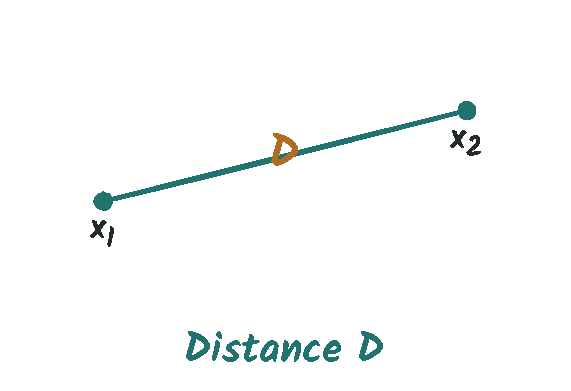
\includegraphics[clip,width=0.31\textwidth,height=19mm,keepaspectratio]{simplex_segment.pdf}\hfill
    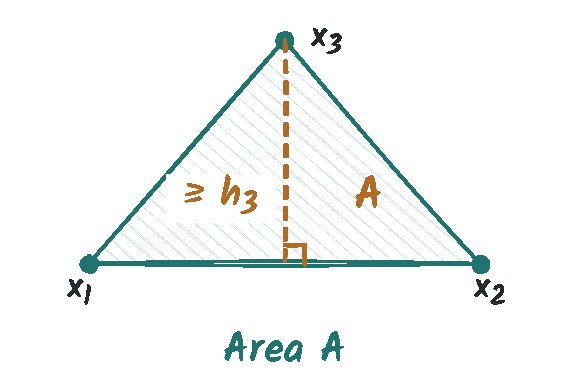
\includegraphics[clip,width=0.31\textwidth,height=19mm,keepaspectratio]{simplex_triangle.pdf}\hfill
    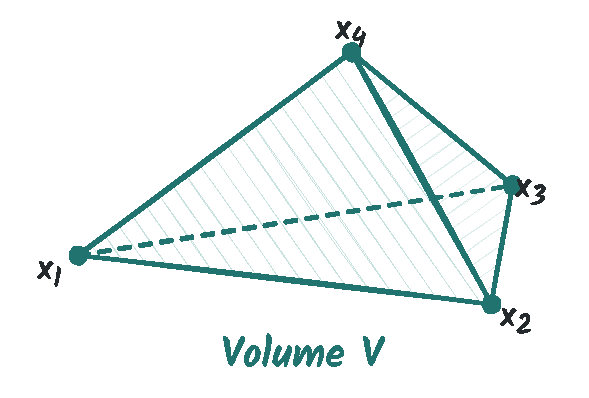
\includegraphics[clip,width=0.31\textwidth,height=19mm,keepaspectratio]{simplex_tetrahedron.pdf}}\par
  \vspace{1mm}
  {\color{assumptionred}\textbf{Additional assumption:}
    require these identities only for diameter $<M$}
  \end{minipage}
  \vspace{2mm}

  \note{Astra6 run 20261020T164437Z\_astra6, statement S1 and proof\_4 v04.
    The construction covers every independently prescribed pair $(\lambda_0,M)>0$.
    The full factorial measures have globally finite-almost-everywhere densities,
    understood as extended nonnegative measures. There is no singular component.
    The normalised identities use $C_n=a_n/\lambda_0^n$.
    There are no positive lower distance, area, volume or altitude thresholds.
    Finite fourth local moments would contradict the reciprocal-volume identity:
    every nonempty ball has infinite fourth moment. Third local moments are finite.
    Unrestricted identities are impossible. A finite diameter cap is the adopted
    restriction, not a uniquely necessary or proved minimal choice.}
\end{frame}

\begin{frame}[t]{\fontsize{18}{22}\selectfont Step 2: configuration/agent files and execution}
  \vspace{1mm}
  \begin{columns}[c,onlytextwidth]
    \begin{column}{0.30\textwidth}
      {\fontsize{11}{13}\selectfont\bfseries Research approaches\par}
      \vspace{3mm}
      {\fontsize{10}{12}\selectfont
      \setbeamercolor{enumerate item}{fg=charcoal}
      \begin{enumerate}
        \setlength{\itemsep}{4mm}
        \item Poisson cluster process
        \item Cox process
        \item Hawkes process
        \item An approach of the agent's choice
        \item Prove non-existence
      \end{enumerate}}
    \end{column}
    \begin{column}{0.68\textwidth}
      \centering
      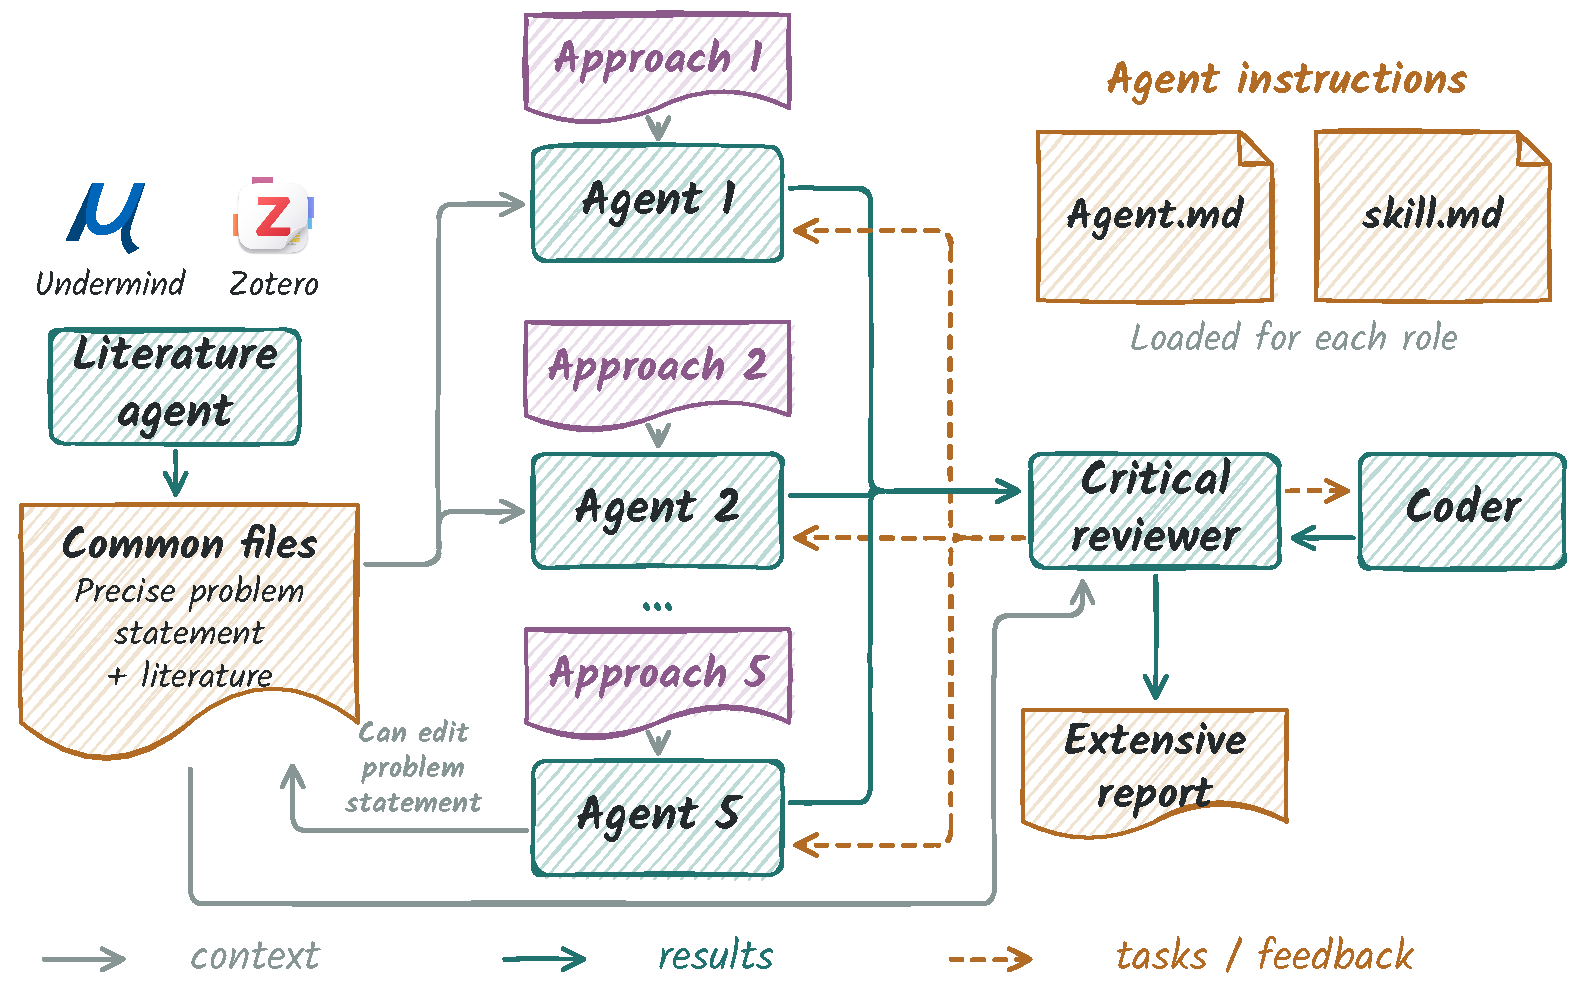
\includegraphics[clip,width=\linewidth,height=59mm,keepaspectratio]{research_agent_configuration.pdf}
    \end{column}
  \end{columns}
\end{frame}

% Slide 16 retained in source, hidden at the owner's request.
% \begin{frame}[t]{Step 3: skills and agents}
%   \noindent{\fontsize{10}{12}\selectfont
%     All agents use \textbf{GPT-5.6 Sol} with \textbf{extra-high} reasoning.\par}
%   \vspace{1mm}
%   \noindent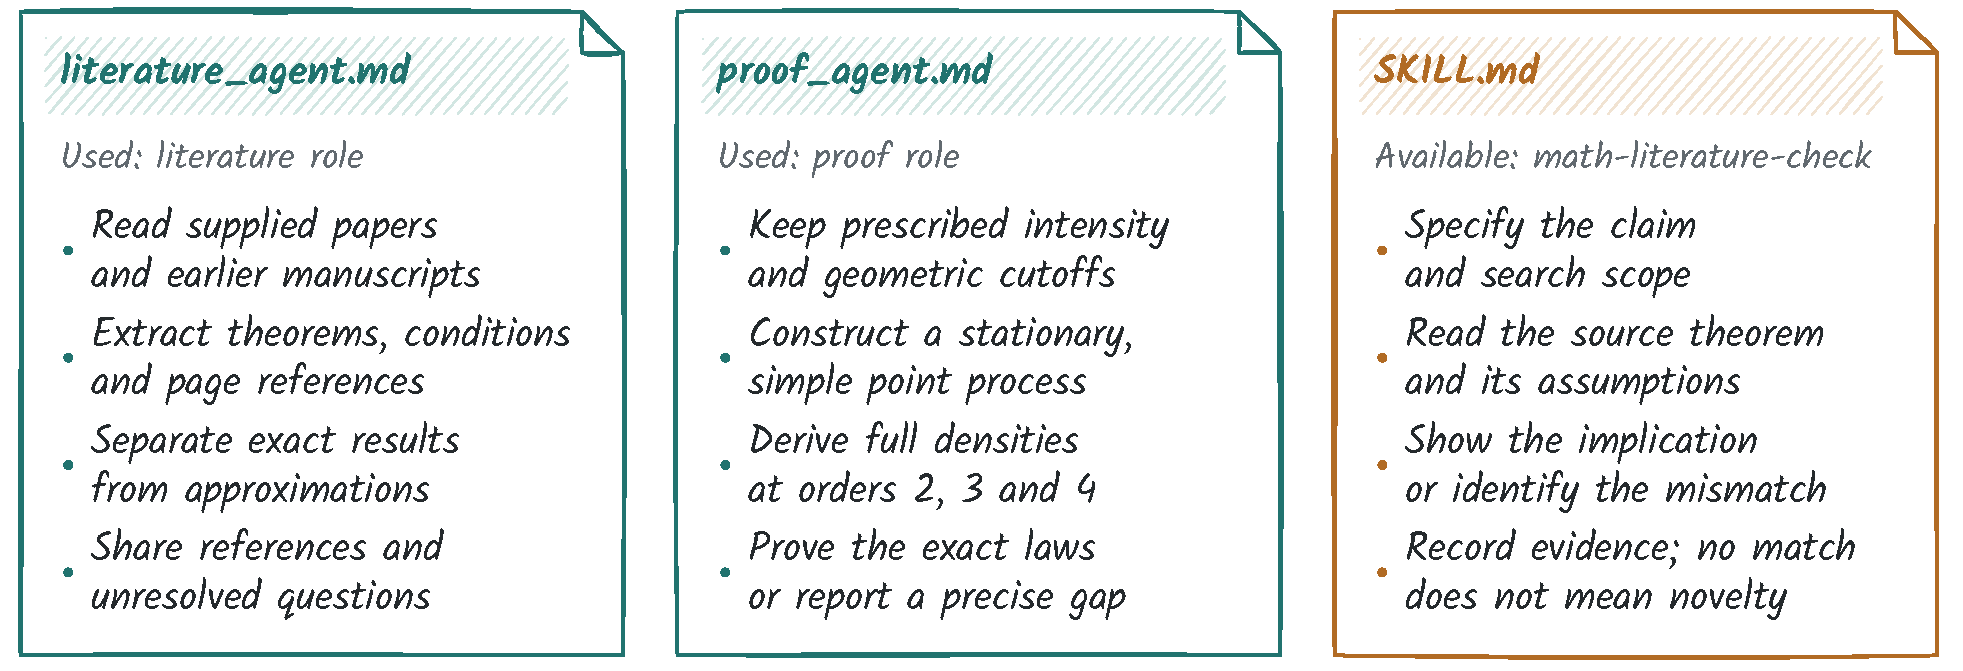
\includegraphics[clip,width=\linewidth,height=49mm,keepaspectratio]{skills_agent_files.pdf}\par
%   \vspace{-1mm}
%   {\fontsize{8}{10}\selectfont
%     \textbf{Instructions matter:} optimising agent prompts can improve
%     mathematical benchmark performance.\par}
%   \vspace{0.8mm}
%   {\fontsize{7}{8.5}\selectfont\color{muted}
%     \href{https://arxiv.org/html/2502.02533v2\#S2.SS1}{Zhou et al. (ICLR 2026), MASS, Section 2.1 and Figure 2: MATH benchmark.}\par}
% \end{frame}

\begin{frame}[t]{Step 3: Writing the paper}
  \vspace{0mm}
  \begin{columns}[T,onlytextwidth]
    \begin{column}{0.50\textwidth}
      \centering
      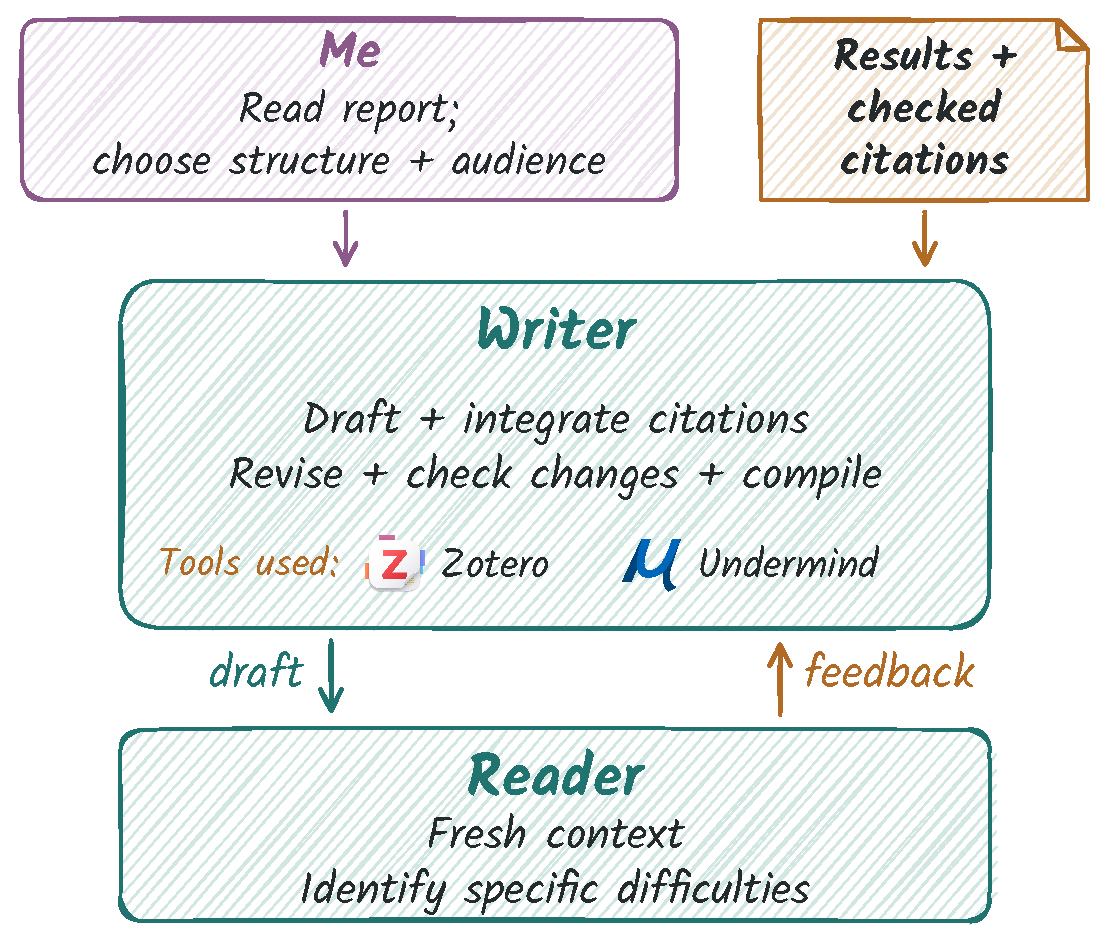
\includegraphics[clip,width=\linewidth,height=37mm,keepaspectratio]{writing_workflow.pdf}\par
  \vspace{2mm}
  {\raggedright\fontsize{8.5}{10}\selectfont
    \begin{itemize}
      \setlength{\itemsep}{1mm}
      \item The paper's appendix also discusses the other approaches.
        They led to interesting ideas, even when they did not work.
      \item The writer gets access to Zotero and Undermind for citations and novelty checks.
    \end{itemize}}

    \end{column}
    \begin{column}{0.47\textwidth}
      {\fontsize{8.5}{10}\selectfont\bfseries Research phase: recorded usage\par}
      \vspace{0.5mm}
      {\fontsize{8.5}{10}\selectfont\color{black}
      \setlength{\tabcolsep}{0pt}
      \renewcommand{\arraystretch}{1.05}
      \begin{tabular*}{\linewidth}{@{}l@{\extracolsep{\fill}}rr@{}}
        \toprule
        \textbf{Work} & \textbf{Tokens (millions)} & \textbf{Est. USD} \\
        \midrule
        Proofer & 69.74 & \$121.04 \\
        Reviewer & 25.94 & \$54.47 \\
        Literature & 3.40 & \$5.65 \\
        \midrule
        \textbf{Total} & \textbf{99.08} & \textbf{\$181.15} \\
        \bottomrule
      \end{tabular*}\par}
      \vspace{1.5mm}
      {\fontsize{8.5}{10}\selectfont\bfseries Writing phase: paper, simulations and review\par}
      \vspace{0.5mm}
      {\fontsize{8}{9.5}\selectfont\color{black}
      \setlength{\tabcolsep}{0pt}
      \renewcommand{\arraystretch}{1.05}
      \begin{tabular*}{\linewidth}{@{}l@{\extracolsep{\fill}}rr@{}}
        \toprule
        \textbf{Token category} & \textbf{Tokens} & \textbf{Est. USD} \\
        \midrule
        Uncached input & 545,555 & \$5.46 \\
        Cached input & 16,615,424 & \$16.62 \\
        Output (incl. reasoning) & 116,258 & \$5.81 \\
        \midrule
        \textbf{Total} & \textbf{17,277,237} & \textbf{\$27.88} \\
        \bottomrule
      \end{tabular*}\par}
      \vspace{0.5mm}
      {\fontsize{6.5}{7.5}\selectfont
        \href{https://developers.openai.com/api/docs/models/gpt-6-astra}{Standard GPT-6-Astra API pricing}.\par}
    \end{column}
  \end{columns}
  \note{Research usage from the Astra6 run, snapshot 20 October 2026.
    Proofer combines the coordinator, both non-existence investigators and all
    four construction tracks. Reviewer combines all 16 submission reviews and
    the final synthesis review. Literature is the literature-check session.
    Exact grouped token counts are 69,740,488; 25,942,234; and 3,395,452.
    Estimated costs sum unrounded source values before rounding to cents:
    USD 121.040184; 54.466436; and 5.648264.
    Total: 99,078,174 tokens and USD 181.154884, displayed as
    99.08 million tokens and USD 181.15.
    Counts include cached input. Cross-session inclusion semantics remain
    unreconciled, and the coordinator snapshot omits its final tail.
    These are recorded-role aggregates and standard API-equivalent estimates,
    not actual account charges or a verified billing total.
    Source: followups/20261020\_cost\_estimate\_v01/cost\_estimate.json
    in run 20261020T164437Z\_astra6.
    Writing-phase usage supplied by the owner: 545,555 uncached input tokens,
    16,615,424 cached input tokens, and 116,258 output tokens including reasoning;
    total 17,277,237 tokens. At standard GPT-6-Astra short-context rates of
    USD 10, 1 and 50 per million tokens respectively, the costs are
    USD 5.455550, 16.615424 and 5.812900, totalling USD 27.883874.
    Displayed line items and the total are rounded independently to cents.
    This is an API-equivalent estimate for writing, simulations and review.
    Pricing checked 21 October 2026:
    \url{https://developers.openai.com/api/docs/models/gpt-6-astra}.}
\end{frame}


\begin{frame}[t]{Results and personal feedback}
  \vspace{-3.5mm}
  \begin{columns}[T,onlytextwidth]
    \begin{column}{0.51\textwidth}
      {\fontsize{11}{13}\selectfont\bfseries Spheres and a cluster correction\par}
      \vspace{1mm}
      {\raggedright\fontsize{8.5}{10}\selectfont
      Idea: I decide between 2 processes with probability $0.5$. Therefore\par
      \noindent\makebox[\linewidth][c]{$\displaystyle
        g_n=\frac{\lambda_A^n g_{n,A}+\lambda_B^n g_{n,B}}{2\lambda_0^n},
        \quad \lambda_0=\frac{\lambda_A+\lambda_B}{2}.$}\par
      \vspace{0.5mm}
      \textbf{Process A.} Takes care of the $g_4 \propto V^{-1}$ by placing non interacting spheres with random radius. A homogeneous Poisson process on this random sphere satisfies $g_4$. We also know $g_3, g_2$ here.  \par
      \vspace{0.5mm}
      \textbf{Process B.} Ensures that $g_{4,B}=0$ for diameter below $M$, using clusters of at most 3 points separated by more than $M$. $g_{2,B}$ and $g_{3,B}$ are designed according to the error in process A via the cluster kernels\par
      \vspace{0.5mm}
      \noindent\makebox[\linewidth][c]{$\displaystyle
        F_3=q_3,\qquad F_2=q_2-\int q_3(\cdot,\cdot,z)\,dz.$}\par
      \vspace{0.5mm}
      Here $q_2,q_3$ are the required product-density corrections.\par}
      \vspace{1mm}
    \end{column}
    \begin{column}{0.46\textwidth}
      {\fontsize{11}{13}\selectfont\bfseries Personal feedback\par}
      \vspace{1mm}
      {\fontsize{8.5}{10}\selectfont
      \setlength{\tabcolsep}{0pt}
      \renewcommand{\arraystretch}{1}
      \begin{tabular}{@{}p{0.69\linewidth}@{\hspace{3mm}}p{0.25\linewidth}@{}}
        \textbf{Aspect} & \textbf{Feedback} \\
        \midrule
        \raggedright Mathematical correctness
          & \textcolor{teal}{Positive}\tabularnewline[0.2mm]
        \raggedright Research and process documentation
          & \textcolor{teal}{Positive}\tabularnewline[0.2mm]
        \raggedright Code writing
          & \textcolor{teal}{Positive}\tabularnewline[0.2mm]
        \raggedright Text writing
          & \textcolor{chartorange}{Medium}\tabularnewline[0.2mm]
        \raggedright Paper structuring
          & \textcolor[HTML]{B04E43}{Negative}\tabularnewline[0.2mm]
        \raggedright Mathematical explanation
          & \textcolor{chartorange}{Medium}\tabularnewline
        \bottomrule
      \end{tabular}\par}
      \vspace{1mm}
      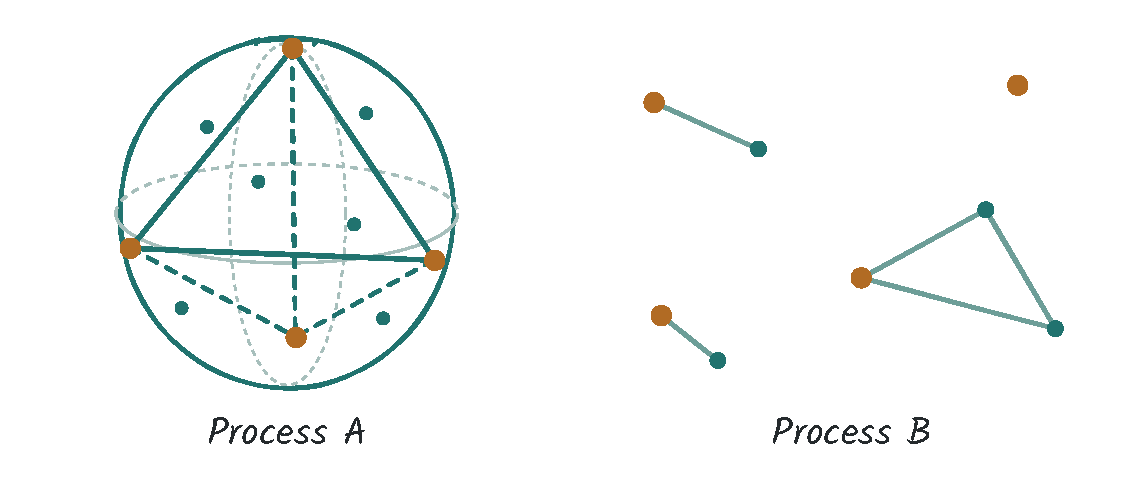
\includegraphics[clip,width=\linewidth,height=29mm,keepaspectratio]{sphere_cluster_mixture.pdf}\par
    \end{column}
  \end{columns}
  \note{Source: Astra6 run 20261020T164437Z\_astra6,
    tracks/proof\_4/submissions/v04.md, Sections 2, 5, 7 and 8,
    and reviews/proof\_4\_v04/review.md.
    A single global fair coin selects the sphere law Y or the correction law C.
    The two point patterns are alternative realisations, not a superposition.
    Conditional on the sphere family, each surface carries an independent
    Poisson process with constant surface intensity a(R)/(2R).
    Distinct sphere surfaces are more than M apart. Four highlighted surface
    points form a tetrahedron, illustrating the circumsphere Jacobian 48V.
    The diagram is schematic and does not prescribe four points per sphere.
    Correction centres come from a Poisson process thinned to separation 3M.
    Size marks are 0, 1, 2 or 3; nonempty clusters contain their centre.
    Their diameter is below M and different clusters are more than M apart.
    F3=q3 and F2=q2 minus the one-vertex marginal of q3.
    In the slide's notation, $q_n=2\lambda_0^n g_n-\lambda_A^n g_{n,A}$
    on the target domain and zero outside, for $n=2,3$.
    The kernels $F_j(0,y_2,\ldots,y_j)$ are divided by their anchored
    integrals $Z_j$ to give the cluster offset densities.
    Thus the correction has local full densities q2, q3 and zero at order four.
    Mixing the two laws gives all three exact reciprocal identities on S1.
    The process has finite third and infinite fourth local moments.}
\end{frame}

\begin{frame}[t]{Future of agentic research}
  \vspace{-1mm}
  \begin{columns}[T,onlytextwidth]
    \begin{column}{0.45\textwidth}
      {\fontsize{10.5}{12}\selectfont\bfseries
        What I expect to change\par}
      \vspace{2mm}
         {\fontsize{8.8}{10.5}\selectfont
        \begin{itemize}
        \setlength{\itemsep}{0.5mm}
            \item  Stronger models can increasingly plan, divide work into tasks,
        use tools and delegate to subagents.
        \item For a precise mathematical problem, one initial prompt may
        increasingly suffice. This can still mean substantial autonomous
        work, with no guarantee of success.
        \item 
        I also expect explanations to become less sloppy and more
        useful for learning.
        \end{itemize}
      \vspace{2mm}}
    \end{column}
    \begin{column}{0.51\textwidth}
      {\fontsize{10.5}{12}\selectfont\bfseries
        Where a custom harness still helps\par}
      \vspace{2mm}
      {\fontsize{8.8}{10.5}\selectfont
      \begin{itemize}
        \setlength{\itemsep}{0.5mm}
        \item Keep the exact target, hypotheses and criteria for success fixed.
        \item Require separate review and formal verification.
        \item Keep human checkpoints for direction and interpretation.
        \item Record results, failed approaches, sources and dependencies.
        \item Set compute budgets, stopping rules and model choice.
        \item When writing papers with AI, set your preferences for writing
          and illustration styles.
      \end{itemize}}
    \end{column}
  \end{columns}
  \vspace{2mm}
  {\color{muted!35}\hrule height 0.4pt}
  \vspace{0.8mm}
  {\fontsize{7.5}{9}\selectfont
    \textbf{A reported example.} Scientific American reports that almost all results in OpenAI's October release
    came from one prompt to one agent. Some may have needed retries;
    the full workflow has not been independently reproduced.\par}
  \vspace{0.6mm}
  {\fontsize{6.5}{7.5}\selectfont\color{muted}
    \href{https://www.scientificamerican.com/article/openai-unleashes-hundreds-more-math-results-upon-a-field-already-in-shock/}{Scientific American, October 2026};
    \href{https://github.com/openai/math\#how-the-results-were-produced}{OpenAI release details}.\par}
\end{frame}

\begin{frame}[t]{Personal take}
  What I have found useful in my research:\par
  \vspace{3mm}
  \begin{itemize}
    \setlength{\itemsep}{3mm}
    \item Writing code.
    \item Managing my literature.
    \item Exploring ideas and proving theorems.
    \item Getting quick new insights.
    \item Visualising my science.
    \item Correcting my writing.
  \end{itemize}
\end{frame}

\begin{frame}[t]{Personal take}
  \vspace{1.5mm}
  \noindent\makebox[\textwidth][c]{%
    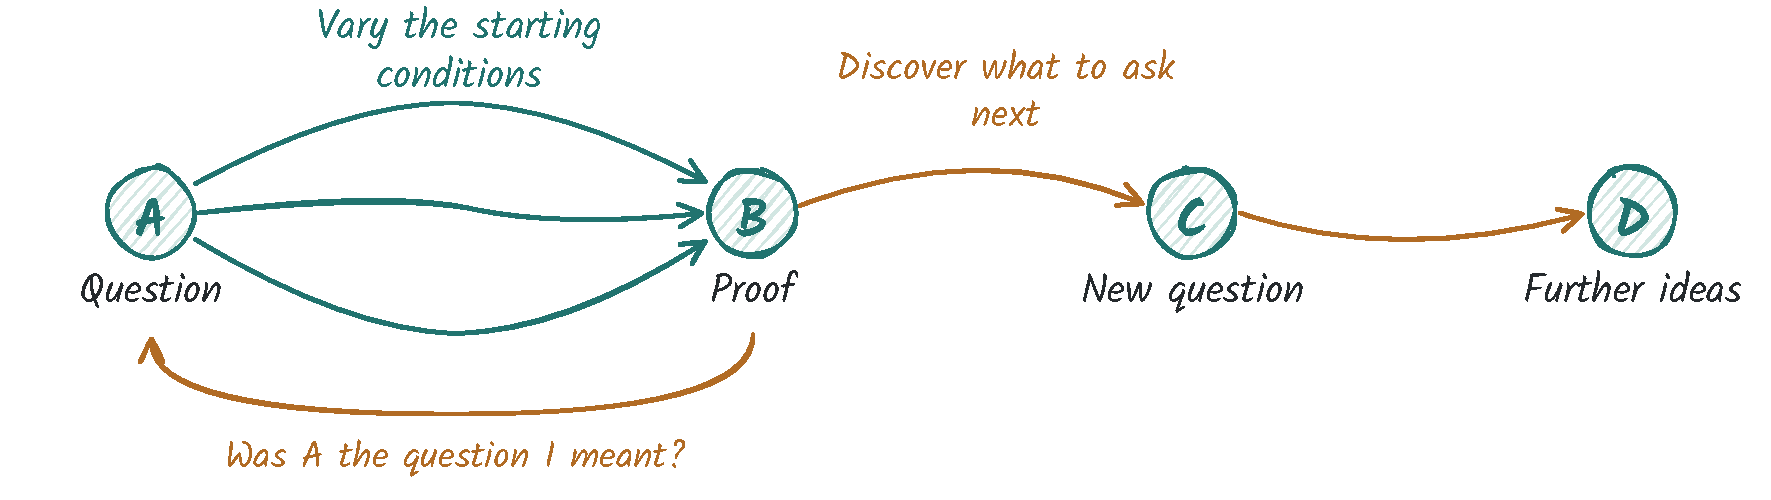
\includegraphics[clip,width=\textwidth,height=31mm,keepaspectratio]{personal_research_paths.pdf}}\par
  \vspace{0.5mm}
  {\fontsize{10}{12}\selectfont
    Reaching $B$ only helps me if I understand the mathematics.\par}
    Reaching $B$ in different ways lets me think about where to go next i.e. $C$. \par
  \vspace{2mm}
  {\fontsize{9}{11}\selectfont
    \textbf{My concern as a PhD student:}
    outsourcing too much may bypass the learning.\par
    A PhD is still an education. Producing results and developing understanding
    can come apart.\par}
  \vspace{1.5mm}
  {\fontsize{6.8}{8}\selectfont\color{muted}
    Related: \href{https://mathandai.org/}{\textit{A Severe Misalignment of AI in Mathematics}}
    (joint declaration, 11 September 2026).\par}
\end{frame}

\begin{frame}[plain]
  \vspace{9mm}
  \begin{columns}[c,onlytextwidth]
    \begin{column}{0.62\textwidth}
      {\fontsize{30}{35}\selectfont\bfseries Thank you!\par}
      \vspace{5mm}
      {\fontsize{14}{17}\selectfont Questions and discussion\par}
      \vspace{9mm}
      {\fontsize{10}{12}\selectfont
        Slides, experiments, documentation and the paper:\par}
      \vspace{2mm}
      {\fontsize{9}{11}\selectfont
        \href{https://github.com/MathisRost/agentic-ai-math}{github.com/MathisRost/agentic-ai-math}\par}
    \end{column}
    \begin{column}{0.33\textwidth}
      \centering
      \href{https://github.com/MathisRost/agentic-ai-math}{%
        
\includegraphics[width=39mm]{repository_qr.pdf}}\par
    \end{column}
  \end{columns}
\end{frame}

\end{document}
